% Options for packages loaded elsewhere
% Options for packages loaded elsewhere
\PassOptionsToPackage{unicode}{hyperref}
\PassOptionsToPackage{hyphens}{url}
\PassOptionsToPackage{dvipsnames,svgnames,x11names}{xcolor}
%
\documentclass[
  11pt,
  a4paper,
  DIV=11,
  numbers=noendperiod]{scrartcl}
\usepackage{xcolor}
\usepackage[lmargin=2.54cm,rmargin=2.54cm,tmargin=2.54cm,bmargin=2.54cm]{geometry}
\usepackage{amsmath,amssymb}
\setcounter{secnumdepth}{5}
\usepackage{iftex}
\ifPDFTeX
  \usepackage[T1]{fontenc}
  \usepackage[utf8]{inputenc}
  \usepackage{textcomp} % provide euro and other symbols
\else % if luatex or xetex
  \usepackage{unicode-math} % this also loads fontspec
  \defaultfontfeatures{Scale=MatchLowercase}
  \defaultfontfeatures[\rmfamily]{Ligatures=TeX,Scale=1}
\fi
\usepackage{lmodern}
\ifPDFTeX\else
  % xetex/luatex font selection
  \setmainfont[]{TeX Gyre Schola}
  \setmonofont[]{Inconsolata}
\fi
% Use upquote if available, for straight quotes in verbatim environments
\IfFileExists{upquote.sty}{\usepackage{upquote}}{}
\IfFileExists{microtype.sty}{% use microtype if available
  \usepackage[]{microtype}
  \UseMicrotypeSet[protrusion]{basicmath} % disable protrusion for tt fonts
}{}
\usepackage{setspace}
\makeatletter
\@ifundefined{KOMAClassName}{% if non-KOMA class
  \IfFileExists{parskip.sty}{%
    \usepackage{parskip}
  }{% else
    \setlength{\parindent}{0pt}
    \setlength{\parskip}{6pt plus 2pt minus 1pt}}
}{% if KOMA class
  \KOMAoptions{parskip=half}}
\makeatother
% Make \paragraph and \subparagraph free-standing
\makeatletter
\ifx\paragraph\undefined\else
  \let\oldparagraph\paragraph
  \renewcommand{\paragraph}{
    \@ifstar
      \xxxParagraphStar
      \xxxParagraphNoStar
  }
  \newcommand{\xxxParagraphStar}[1]{\oldparagraph*{#1}\mbox{}}
  \newcommand{\xxxParagraphNoStar}[1]{\oldparagraph{#1}\mbox{}}
\fi
\ifx\subparagraph\undefined\else
  \let\oldsubparagraph\subparagraph
  \renewcommand{\subparagraph}{
    \@ifstar
      \xxxSubParagraphStar
      \xxxSubParagraphNoStar
  }
  \newcommand{\xxxSubParagraphStar}[1]{\oldsubparagraph*{#1}\mbox{}}
  \newcommand{\xxxSubParagraphNoStar}[1]{\oldsubparagraph{#1}\mbox{}}
\fi
\makeatother


\usepackage{longtable,booktabs,array}
\usepackage{calc} % for calculating minipage widths
% Correct order of tables after \paragraph or \subparagraph
\usepackage{etoolbox}
\makeatletter
\patchcmd\longtable{\par}{\if@noskipsec\mbox{}\fi\par}{}{}
\makeatother
% Allow footnotes in longtable head/foot
\IfFileExists{footnotehyper.sty}{\usepackage{footnotehyper}}{\usepackage{footnote}}
\makesavenoteenv{longtable}
\usepackage{graphicx}
\makeatletter
\newsavebox\pandoc@box
\newcommand*\pandocbounded[1]{% scales image to fit in text height/width
  \sbox\pandoc@box{#1}%
  \Gscale@div\@tempa{\textheight}{\dimexpr\ht\pandoc@box+\dp\pandoc@box\relax}%
  \Gscale@div\@tempb{\linewidth}{\wd\pandoc@box}%
  \ifdim\@tempb\p@<\@tempa\p@\let\@tempa\@tempb\fi% select the smaller of both
  \ifdim\@tempa\p@<\p@\scalebox{\@tempa}{\usebox\pandoc@box}%
  \else\usebox{\pandoc@box}%
  \fi%
}
% Set default figure placement to htbp
\def\fps@figure{htbp}
\makeatother


% definitions for citeproc citations
\NewDocumentCommand\citeproctext{}{}
\NewDocumentCommand\citeproc{mm}{%
  \begingroup\def\citeproctext{#2}\cite{#1}\endgroup}
\makeatletter
 % allow citations to break across lines
 \let\@cite@ofmt\@firstofone
 % avoid brackets around text for \cite:
 \def\@biblabel#1{}
 \def\@cite#1#2{{#1\if@tempswa , #2\fi}}
\makeatother
\newlength{\cslhangindent}
\setlength{\cslhangindent}{1.5em}
\newlength{\csllabelwidth}
\setlength{\csllabelwidth}{3em}
\newenvironment{CSLReferences}[2] % #1 hanging-indent, #2 entry-spacing
 {\begin{list}{}{%
  \setlength{\itemindent}{0pt}
  \setlength{\leftmargin}{0pt}
  \setlength{\parsep}{0pt}
  % turn on hanging indent if param 1 is 1
  \ifodd #1
   \setlength{\leftmargin}{\cslhangindent}
   \setlength{\itemindent}{-1\cslhangindent}
  \fi
  % set entry spacing
  \setlength{\itemsep}{#2\baselineskip}}}
 {\end{list}}
\usepackage{calc}
\newcommand{\CSLBlock}[1]{\hfill\break\parbox[t]{\linewidth}{\strut\ignorespaces#1\strut}}
\newcommand{\CSLLeftMargin}[1]{\parbox[t]{\csllabelwidth}{\strut#1\strut}}
\newcommand{\CSLRightInline}[1]{\parbox[t]{\linewidth - \csllabelwidth}{\strut#1\strut}}
\newcommand{\CSLIndent}[1]{\hspace{\cslhangindent}#1}



\setlength{\emergencystretch}{3em} % prevent overfull lines

\providecommand{\tightlist}{%
  \setlength{\itemsep}{0pt}\setlength{\parskip}{0pt}}



 


\KOMAoption{captions}{tableheading}
\makeatletter
\@ifpackageloaded{caption}{}{\usepackage{caption}}
\AtBeginDocument{%
\ifdefined\contentsname
  \renewcommand*\contentsname{Table of contents}
\else
  \newcommand\contentsname{Table of contents}
\fi
\ifdefined\listfigurename
  \renewcommand*\listfigurename{List of Figures}
\else
  \newcommand\listfigurename{List of Figures}
\fi
\ifdefined\listtablename
  \renewcommand*\listtablename{List of Tables}
\else
  \newcommand\listtablename{List of Tables}
\fi
\ifdefined\figurename
  \renewcommand*\figurename{Figure}
\else
  \newcommand\figurename{Figure}
\fi
\ifdefined\tablename
  \renewcommand*\tablename{Table}
\else
  \newcommand\tablename{Table}
\fi
}
\@ifpackageloaded{float}{}{\usepackage{float}}
\floatstyle{ruled}
\@ifundefined{c@chapter}{\newfloat{codelisting}{h}{lop}}{\newfloat{codelisting}{h}{lop}[chapter]}
\floatname{codelisting}{Listing}
\newcommand*\listoflistings{\listof{codelisting}{List of Listings}}
\makeatother
\makeatletter
\makeatother
\makeatletter
\@ifpackageloaded{caption}{}{\usepackage{caption}}
\@ifpackageloaded{subcaption}{}{\usepackage{subcaption}}
\makeatother
\usepackage{bookmark}
\IfFileExists{xurl.sty}{\usepackage{xurl}}{} % add URL line breaks if available
\urlstyle{same}
\hypersetup{
  pdftitle={Did England Deserve to Win? A Data Dashboard Analysis of UEFA Women's Euro 2025},
  pdfauthor={Janine Buergler (201944190)},
  colorlinks=true,
  linkcolor={blue},
  filecolor={Maroon},
  citecolor={Blue},
  urlcolor={Blue},
  pdfcreator={LaTeX via pandoc}}


\title{Did England Deserve to Win? A Data Dashboard Analysis of UEFA
Women's Euro 2025}
\author{Janine Buergler (201944190)}
\date{2026-05-09}
\begin{document}
\maketitle

\renewcommand*\contentsname{Table of contents}
{
\hypersetup{linkcolor=}
\setcounter{tocdepth}{3}
\tableofcontents
}
\listoffigures
\listoftables

\setstretch{1.15}
\textbf{Live dashboard:}
\url{https://jbuergler.github.io/football-analytics/}

\textbf{Repository:}
\url{https://github.com/jbuergler/football-analytics}

\newpage{}

\section{Introduction and Research
Question}\label{introduction-and-research-question}

The UEFA Women's European Championship (Euro) is one of the most
important tournaments in women's football. The 2025 edition, hosted in
in Switzerland from 2nd to 27th July 2025, came at a moment when the
sport continues to grow in visibility, commercial value and public
attention. The tournament has achieved record television audiences in
the United Kingdom (Women's Sport Trust, 2026). Sixteen nations competed
across the group stage and knockout rounds, producing 106 goals across
31 matches and setting multiple tournament records (UEFA, 2025d).(UEFA,
2025c).

Research on women's football shows that this growth is part of a broader
professionalisation, but that major gaps between the women's and men's
game remain in areas such as commercial investment, media coverage, and
resources (Tjønndal \emph{et al.}, 2024). This makes the tournament
interesting not just because of who won, but about whether performance
data supports the results. This is something that matters to fans,
analysts, journalists, coaches, and anyone interested in how women's
football is judged and valued.

The tournament ended with the final match at St.~Jakob on the 27th of
July 2025, where England faced Spain. England entered the tournament as
the defending title holders, whereas Spain were the reigning World Cup
holders. Spain's Aitana Bonmatí was named Player of the Tournament,
while Esther González finished as the tournament's top scorer with four
goals (UEFA, 2025c, 2025a). (UEFA, 2025d, 2025a). Following a 1-1 draw
after extra time, England won 3-1 on penalties to retain their European
title (Sanders, 2025).

(Sanders, 2025).

The result, however, raised an immediate analytical question: did the
scoreline reflect the balance of the play throughout the tournament and
in the final itself? This project uses StatsBomb open event data to
directly compare England and Spain's performances across the tournament
and in the final itself, through metrics including expected goals (xG),
pressing intensity, and ball progression. The central research question
is:

\textbf{Did England deserve to win the Women's Euro 2025?}

This question matters because women's football is undergoing clear
professionalisation, yet there are still major gaps with the men's game
regarding visibility, financial conditions, and commercial value
(Tjønndal \emph{et al.}, 2024). Recent research also shows that
professional women's football has evolved technically and tactically,
with event data revealing longer possession sequences, fewer
long-distance shots, and more difficult, valuable passes (Bransen and
Davis, 2024). This makes event data a useful basis for assessing whether
the result reflected the balance of play. For that reason, this project
evaluates whether England's title win in 2025 was deserved on
performance as well as on the scoreboard.

\section{Data Collection and
Preparation}\label{data-collection-and-preparation}

\subsection{Source and Access}\label{source-and-access}

For this project, event data for the UEFA Women's EURO 2025 was sourced
via the \texttt{StatsBombR} package in R (Hudl, no date). Recently,
StatsBomb was incorporated into Hudl's industry-leading ecosystem of
integrated video and analytic solutions (Hudl Statsbomb, 2024). They are
an established provider of football event data, recording over 3,400
events per match across more than 190 competitions and thus providing a
wide range of data free of charge (Hudl Statsbomb, no date). Key
functions including \texttt{allclean()} for enriching event coordinates
and pass end locations followed the workflow outlined in the Working
with R guide (StatsBomb, 2022, p. 25).

\subsection{Dataset Structure and
Granularity}\label{dataset-structure-and-granularity}

The raw data is structured at the event level, meaning that each row
represents a single action during a match. This includes actions such as
passes, carries, shots, pressures, and ball receipts. Each event has
information on the player, team, match, time, pitch location (x, y
coordinates), and action-specific attributes such as shot outcome and xG
value for shots. The x and y coordinates follow the StatsBomb (2019, p.
34) coordinate system where the pitch runs from 0 to 120 on the x-axis
and 0 to 80 on the y-axis. The full dataset covers 31 matches across the
group stage and knockout rounds, including 875 shots after cleaning. Key
variables used in this analysis include:

\begin{itemize}
\item
  \textbf{location\_x, location\_y:} pitch coordinates of the action
\item
  \textbf{shot.statsbomb.xg:} expected goals value for each shot
\item
  \textbf{shot.outcome.name:} outcome of the shot (goal, saved, off
  target, etc.)
\item
  \textbf{type.name:} event type (shot, pass, carry, pressure, etc.)
\item
  \textbf{team.name:} the team performing the action
\item
  \textbf{player.name:} the player performing the action
\item
  \textbf{minute, period:} time context of the action
\end{itemize}

\subsection{Cleaning and Preparation}\label{cleaning-and-preparation}

Several cleaning steps were applied to prepare the data for the
analysis:

\textbf{Period filter:} StatsBomb records penalty shootouts as period 5.
As penalty shootouts are based on individual shots rather than open play
performance, all period 5 events were excluded from the analysis. This
affected a total of three matches: the Sweden vs England semi-final, the
France vs Germany quarter final, and the England vs Spain final.

\textbf{Own goals:} Own goals were excluded from the shot and xG
analysis as they do not reflect the performance of the attacking team.
This means goals from the analytical shot count (875 shots) differs
slightly from the total goals shown in the dashboard (103 vs 106).

\textbf{Team name standardisation:} Team names were cleaned and
standardised to ensure consistency across all tables and visualisations.
Prefixes and Suffixes like ``Women's'' or ``WNT'' (for Finland) were
removed.

\textbf{Pre-aggregation:} Summary tables for the different metrics
analysed in this project were computed in advance and saved as
\texttt{.rds} files. They are loaded directly by the Shiny dashboard.
This approach improves loading speed and separates the data preparation
from the app itself.

\subsection{Coverage and Caveats}\label{coverage-and-caveats}

As shown in Table~\ref{tbl-data-summary}, the dataset covers all 31
matches of the UEFA Women's Euro 2025 tournament from the group stage
through to the final. As coverage is subject to StatsBomb's data
collection methodology, any recording errors cannot be ruled out.

This project analysed on-ball actions only. Off-ball movements and
physical metrics such as distance covered are not included. This means
that some aspects of performance, especially defensive organisation away
from the ball, were not covered in this analysis. StatsBomb's freeze
frame data, which records the location of all players involved in the
event, including goalkeeper and defender positions at the moment of each
shot was not used in this analysis (Hudl Statsbomb, 2021). However, it
informed the pre-computed xG values available in the dataset, which
makes them more contextually accurate. This directly represents a
potential aspect, that future work could incorporate in the analysis.
Across the full dataset, a total of 105,525 individual events were
recorded.

StatsBomb records concrete pressing events when a player applies
pressure to an opponent in possession, instead of computing pressure
through combining multiple defensive actions (Dorrington, 2025). This is
an advantage, as it allows pressing intensity to be evaluated directly
from recorded events.

\begin{longtable}[]{@{}
  >{\raggedright\arraybackslash}p{(\linewidth - 2\tabcolsep) * \real{0.2405}}
  >{\raggedright\arraybackslash}p{(\linewidth - 2\tabcolsep) * \real{0.7595}}@{}}

\caption{\label{tbl-data-summary}Dataset Summary - UEFA Women's Euro
2025}

\tabularnewline

\toprule\noalign{}
\begin{minipage}[b]{\linewidth}\raggedright
Item
\end{minipage} & \begin{minipage}[b]{\linewidth}\raggedright
Detail
\end{minipage} \\
\midrule\noalign{}
\endhead
\bottomrule\noalign{}
\endlastfoot
Source & StatsBomb open event data \\
Access method & StatsBomb R package \\
Competition & UEFA Women's Euro 2025 (ID: 53, Season: 315) \\
Matches & 31 \\
Shots & 875 \\
Granularity & Event level (one row per action), a total of 105,525
events \\
Period 5 excluded & Yes (penalty shootouts) \\
Own goals excluded & Yes (from xG analysis) \\

\end{longtable}

\section{Methodology}\label{methodology}

\subsection{From Raw Data to
Dashboard}\label{from-raw-data-to-dashboard}

This project follows a structured pipeline of five scripts, moving from
raw data collection through to the interactive dashboard. Raw event data
was pulled from StatsBomb in script \texttt{01\_data.R}, explored in
\texttt{02\_explore.R}, cleaned in \texttt{03\_clean.R}, aggregated into
summary tables in \texttt{04\_analyse.R}, and visualised in
\texttt{05\_visualise.R}. As a first step, only the planned static
visuals were created, before moving them as interactive elements in
\texttt{app/app.R}. After the app successfully ran locally on R, it was
then deployed as the dashboard itself via Shinylive to GitHub. This
ensures the analysis is reproducible and the dashboard only uses
smaller, cleaned data tables, that are easier to load through Shiny.

\subsection{Metrics}\label{metrics}

All metrics were computed from the cleaned event data and aggregated
into summary tables. The following metrics were used across the
dashboard:

\textbf{Expected goals difference (xG diff):} For each match, xG
difference was calculated as a team's total xG minus their opponent's
total xG. Averaging this across all matches gives a tournament-wide
measure to see whether a team consistently created better chances than
they conceded. This is the primary metric for the Tournament Overview
tab of the Dashboard.

\textbf{High press rate:} The high press rate was defined as the
proportion of all pressure events happening in the opponent's half of
the pitch (\texttt{location\_x\ \textgreater{}\ 60} on the StatsBomb
coordinate system). StatsBomb records a pressure event each time a
player actively applies pressure to an opponent in possession, which is
a direct measure of pressing behaviour.

\textbf{Counter-press rate:} The counter-press rate was defined as the
proportion of events that StatsBomb flagged as counter pressing. This
refers to pressures applied within a short window of losing the ball.
Missing values were recoded to \texttt{FALSE} so the full pressure count
could be used to compute the rate in \%.

\textbf{Pass completion rate:} The proportion of attempted passes that
successfully reached a teammate from all open play passes. Unknown
outcomes and injury clearances from \texttt{pass.outcome.name} were
excluded. It is worth noting that in the StatsBomb data, \texttt{NA}
values in \texttt{pass.outcome.name} refer to completed passes
(StatsBomb, 2019, p. 28).

\textbf{Final third carry rate:} This refers to the proportion of all
carries ending beyond \texttt{x\ =\ 80} on the StatsBomb coordinate
system, which represents the final third of the pitch. This metric was
chosen over the standard StatsBomb progressive carry definition (carries
advancing the ball by at least 10 units). As it directly shows
penetration into the attacking third instead of forward progress from
any location, this was chosen as a more meaningful metric to analyse the
attacking play.

\textbf{Final third pass rate:} The proportion of completed passes that
ended beyond \texttt{x\ =\ 80} to measure how frequently each team moved
the ball into the attacking third through passing.

\textbf{Shots faced per match:} The average number of shots conceded per
match, used as a measure for defensive solidity alongside average xG
conceded.

\subsection{Grouping and Filtering
Decisions}\label{grouping-and-filtering-decisions}

All pressing metrics were split by stage type (group stage vs knockout
rounds) to capture if there were any tactical shifts as the tournament
progressed. The final match was isolated by selecting only the match ID
of the final itself using \texttt{competition\_stage\ ==\ "Final"} and
analysed separately across the tabs that focused on a detailed analysis
of the events in the final between England and Spain. Actions of the
best players were filtered to Bonmatí and Hemp specifically. They
accumulated the most final third passes and carries for their teams. The
pass map visualisation follows the approach outlined in the Working with
R guide by StatsBomb (2022, pp. 22--24).

\subsection{Dashboard Design}\label{dashboard-design}

The dashboard was built using R Shiny with the \texttt{bslib} package
for the layout and theme (Sievert, 2023). A consistent colour palette
was applied for the entire dashboard based on the official hex colours
of Spain in gold (\texttt{\#F1BF00}) and England in red
(\texttt{\#CE1124}). All other teams were highlighted in grey to ensure
England and Spain can be immediately identified across every chart.

The dashboard was structured across a total of six tabs that guides the
reader through the story of the tournament and ultimately answering the
research question. First, Tournament Facts and Context was provided
about the competition itself, as well as manager, formation, and
high-performing player information for England and Spain. After that,
the Tournament Overview provided context of the team's performance
regarding their expected goals (scored and conceded). Moving on, the
Journey Tab shows the development of the two finalists throughout the
tournament across metrics like accumulated xG, match-by-match xG and
pressing. Afterwards, the final was analysed in more detail across two
tabs to analyse the shot and xG situation, as well as the Possession in
separate windows. The final was split across two tabs deliberately, as
otherwise the plots would be too visually cluttered and overwhelming.
Finally, an analytical decision was made based on the analysed metrics
to answer the research question. This ensures that the reader is guided
from a broad to specific context. Each tab includes a navigation sidebar
that can be collapsed if need be, to give some initial context of what
each tab is trying to show. A preview of the Dashboard can be found in
Appendix A.

The individual chart types were chosen based on the analytical question
each visualisation attempted to address. A horizontal bar chart (Tab 1)
ranks all 16 teams by xG dominance, making the ranking immediately
readable. A scatter plot (Tab 1) compares total xG against goals scored,
showing which teams over- or underperformed in terms of goals.
Cumulative line charts show how the xG and momentum changes across the
tournament, while step charts show the xG accumulated shot by shot in
the final. Pitch-based plots like shot maps (scatter plot) and player
passmaps (arrow maps) use spatial data to show where on the pitch
certain actions happened. Reference lines at +1 and -1 are added to the
xG ranking chart to provide context to what refers to a meaningfully
positive or negative xG difference per match.

Apart from two exceptions, all plotly charts include hover tooltips
providing exact values for each elements of the plots. The xG Dominance
ranking chart and player passmaps use static \texttt{renderPlot} instead
of \texttt{plotly}. For the passmaps, this was due to a compatibility
constraint between the \texttt{ggsoccer} package and the rendering
mechanism of \texttt{plotly} in the Shinylive WebAssembly environment.
For the xG ranking chart, the static approach was chosen, as
interactivity does not add meaningful value to a ranked chart. The
relative positions and reference lines at ±1 communicate the findings
clearly without tooltips.

\section{Findings}\label{findings}

\subsection{Tournament Picture}\label{tournament-picture}

As shown in Figure~\ref{fig-xg-ranking} both England and Spain
outperformed their expected goals across the tournament. Spain scored 18
goals from 15.91 xG (+2.09) and England scored 16 goals from 14.68 xG
(+1.32). This suggests that both teams were clinical in front of goal,
with Spain being slightly more clinical and also generating more chance
quality.

\begin{figure}

\centering{

\pandocbounded{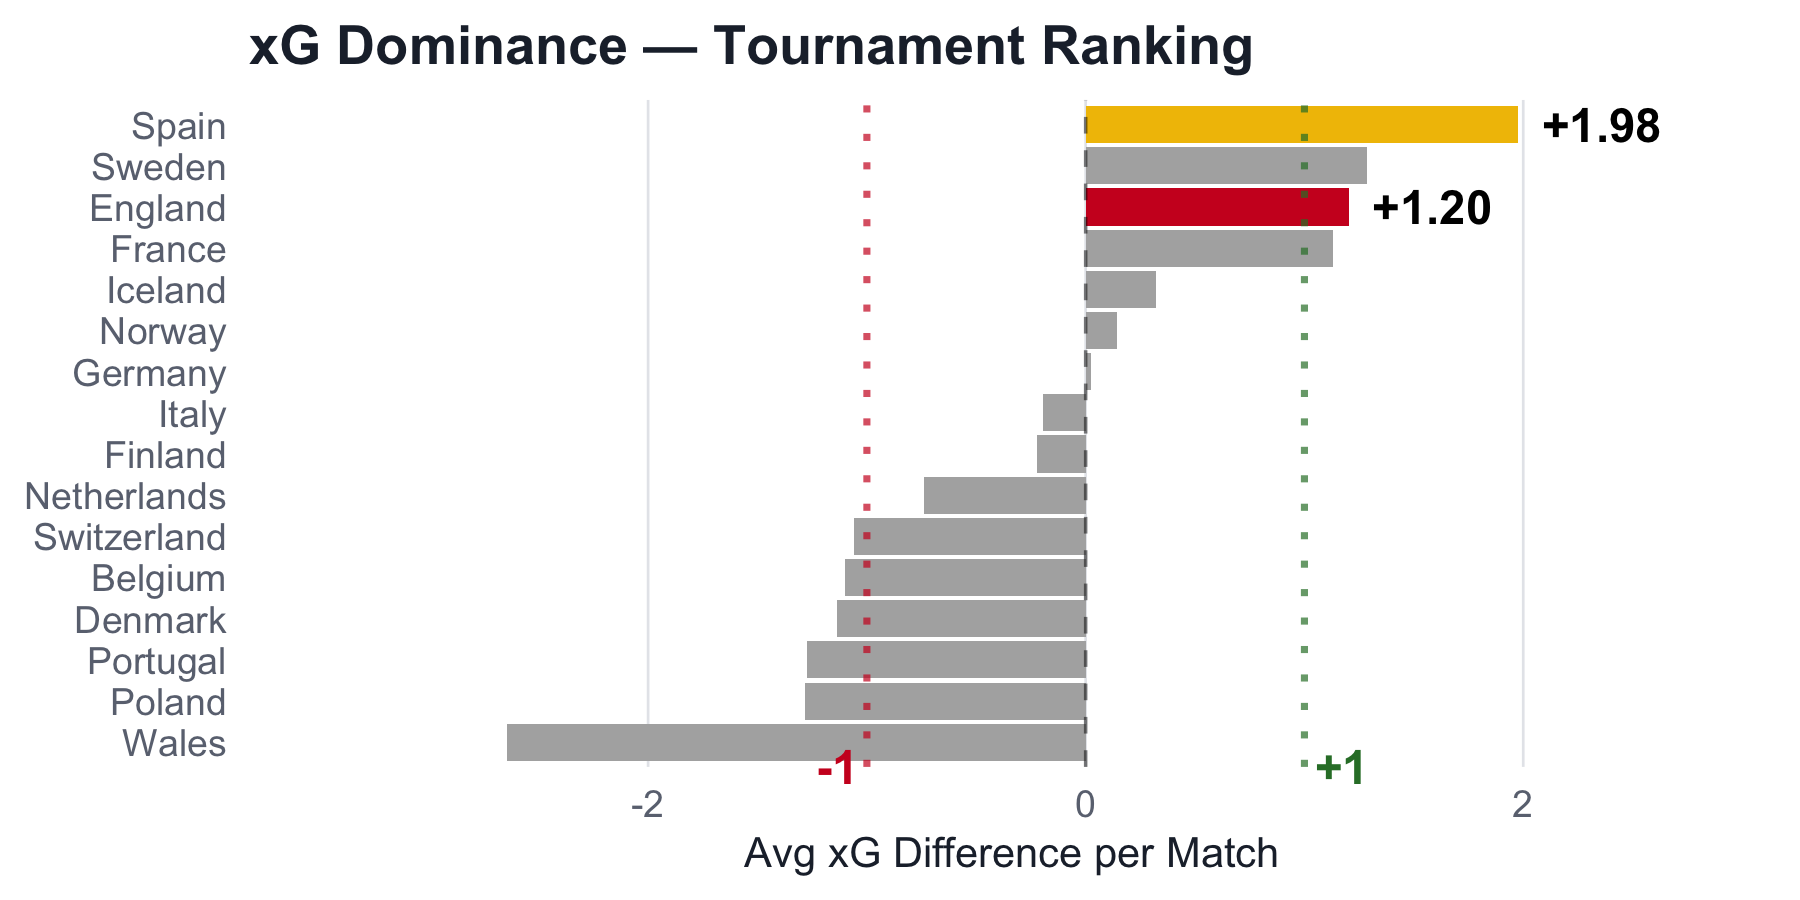
\includegraphics[keepaspectratio]{Report_files/figure-pdf/fig-xg-ranking-1.png}}

}

\caption{\label{fig-xg-ranking}xG Dominance Tournament Ranking --- all
16 teams ranked by average xG difference per match. Spain led the
tournament (+1.98), ahead of England (+1.20).}

\end{figure}%

Looking at the average xG difference in Figure~\ref{fig-xg-scatter},
Spain outperformed all other teams, having an average xG difference of
+1.98 per match. This means that across all their six matches, they
created significantly better chances than they conceded. England came
third, having an average xG difference of +1.20 per match, just behind
Sweden. This figure shows that both teams who reached the final
performed above the +1 reference line, creating more quality chances in
attack than conceding them. Wales had the lowest average xG difference
per match (-2.65), which is reflected in their early group stage exit.
However, this number is slightly inflated, due to their 1-6 loss against
England on Matchday 3.

\begin{figure}

\centering{

\pandocbounded{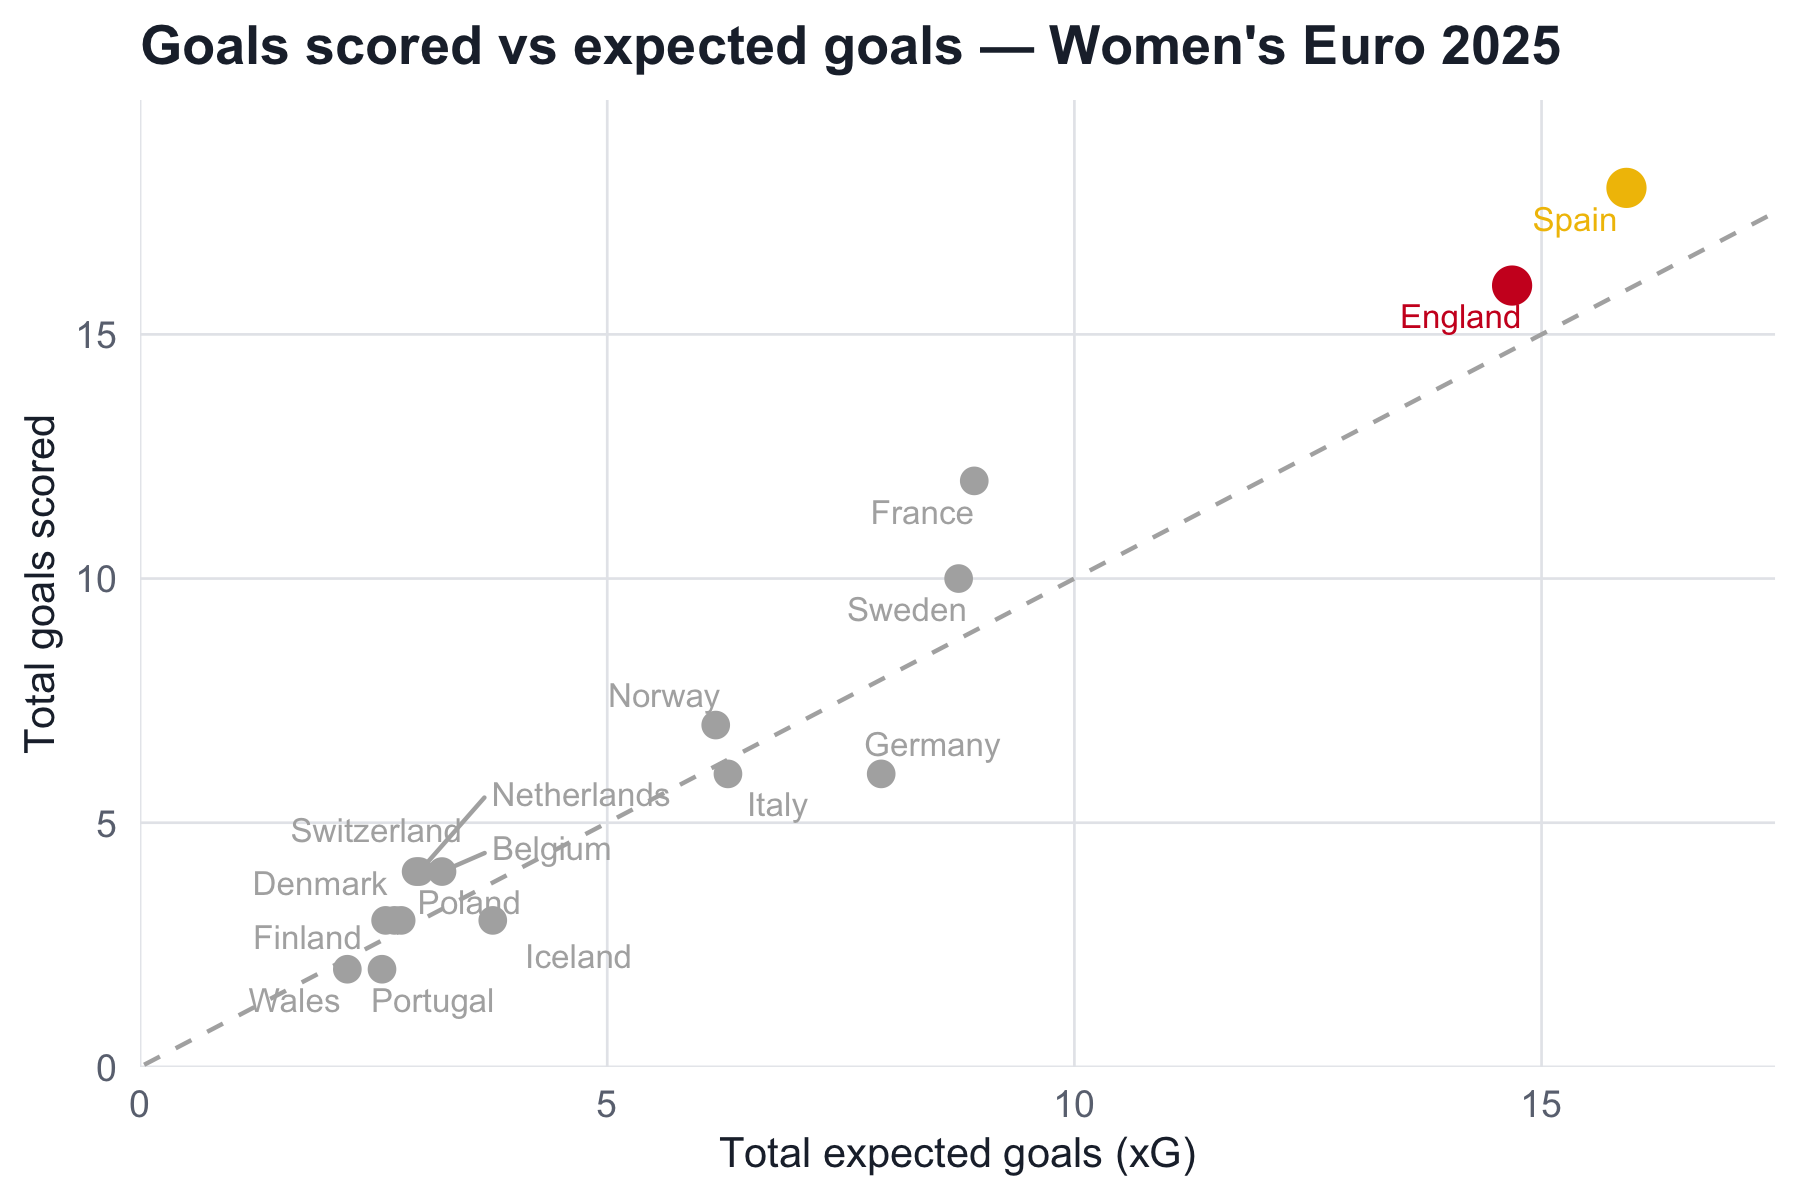
\includegraphics[keepaspectratio]{Report_files/figure-pdf/fig-xg-scatter-1.png}}

}

\caption{\label{fig-xg-scatter}Goals scored vs total xG for all 16
teams. Teams above the dashed line scored more than expected and teams
below the dashed line scored less than expected. Both England and Spain
outperformed their xG, with Spain generating greater overall chance
quality.}

\end{figure}%

\subsection{The Journey to the Final}\label{the-journey-to-the-final}

To compare England's and Spain's routes to the final and how they
performed one by one until playing each other in Basel, several metrics
were analysed.

Figure~\ref{fig-cumulative-xg} shows how both teams' cumulative xG
increased over the whole tournament. The data shows that Spain had a
consistent increase in xG, whereas England had a big increase on
Matchday 3, due to their 6-1 win against Wales. Over the rest of the
tournament both teams' values were at \textasciitilde{} 13.80 after the
semi-finals, before Spain taking the lead after the final on July 27th.
The overall difference, is at +1.23 for Spain. Overall, the figure shows
that Spain had a more consistent attacking output throughout the
tournament compared to England.

\begin{figure}

\centering{

\pandocbounded{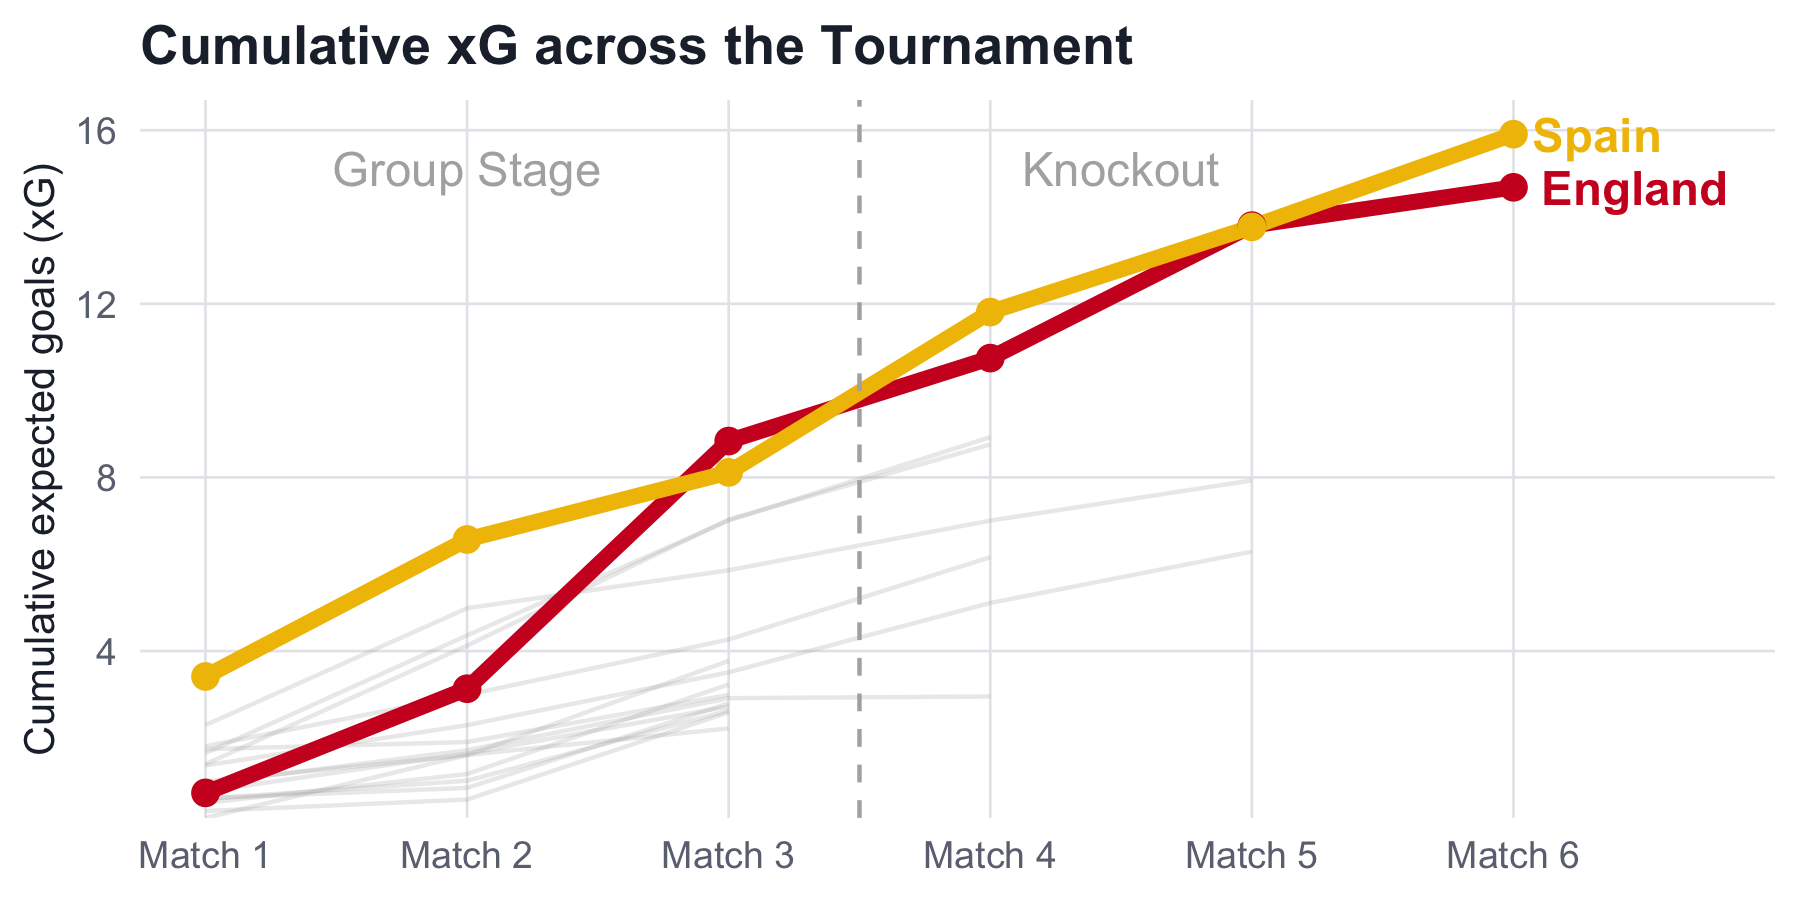
\includegraphics[keepaspectratio]{Report_files/figure-pdf/fig-cumulative-xg-1.png}}

}

\caption{\label{fig-cumulative-xg}Cumulative xG across the tournament
for England and Spain. Spain built xG at a consistently higher rate,
pulling clear from Match 4 onwards. Grey lines show all other teams.}

\end{figure}%

Figure~\ref{fig-pressing} shows the pressing intensity across high
pressing and counter pressing. Evaluating both these metrics, Spain is
ahead of England in the group stages and knockouts. They achieved their
highest rates in the group stages with 76.6\% (high-press rate) and
32.3\% (counter-press rate). This reflects Spain's tactical approach of
high-intensity, ball-oriented pressing. The data, however, shows that
Spain in particular, reduced their pressing intensity in the knockouts,
compared to the group stages. This is not surprising, considering the
margins to win in the knockouts are usually higher, and a pressing done
wrong could lead to a fatal counterattack. Surprisingly, England's
counter pressing only marginally reduced in the later stages of the
tournament (-2.50\%). This shows that there was a smaller tactical
change compared to Spain.

\begin{figure}

\centering{

\pandocbounded{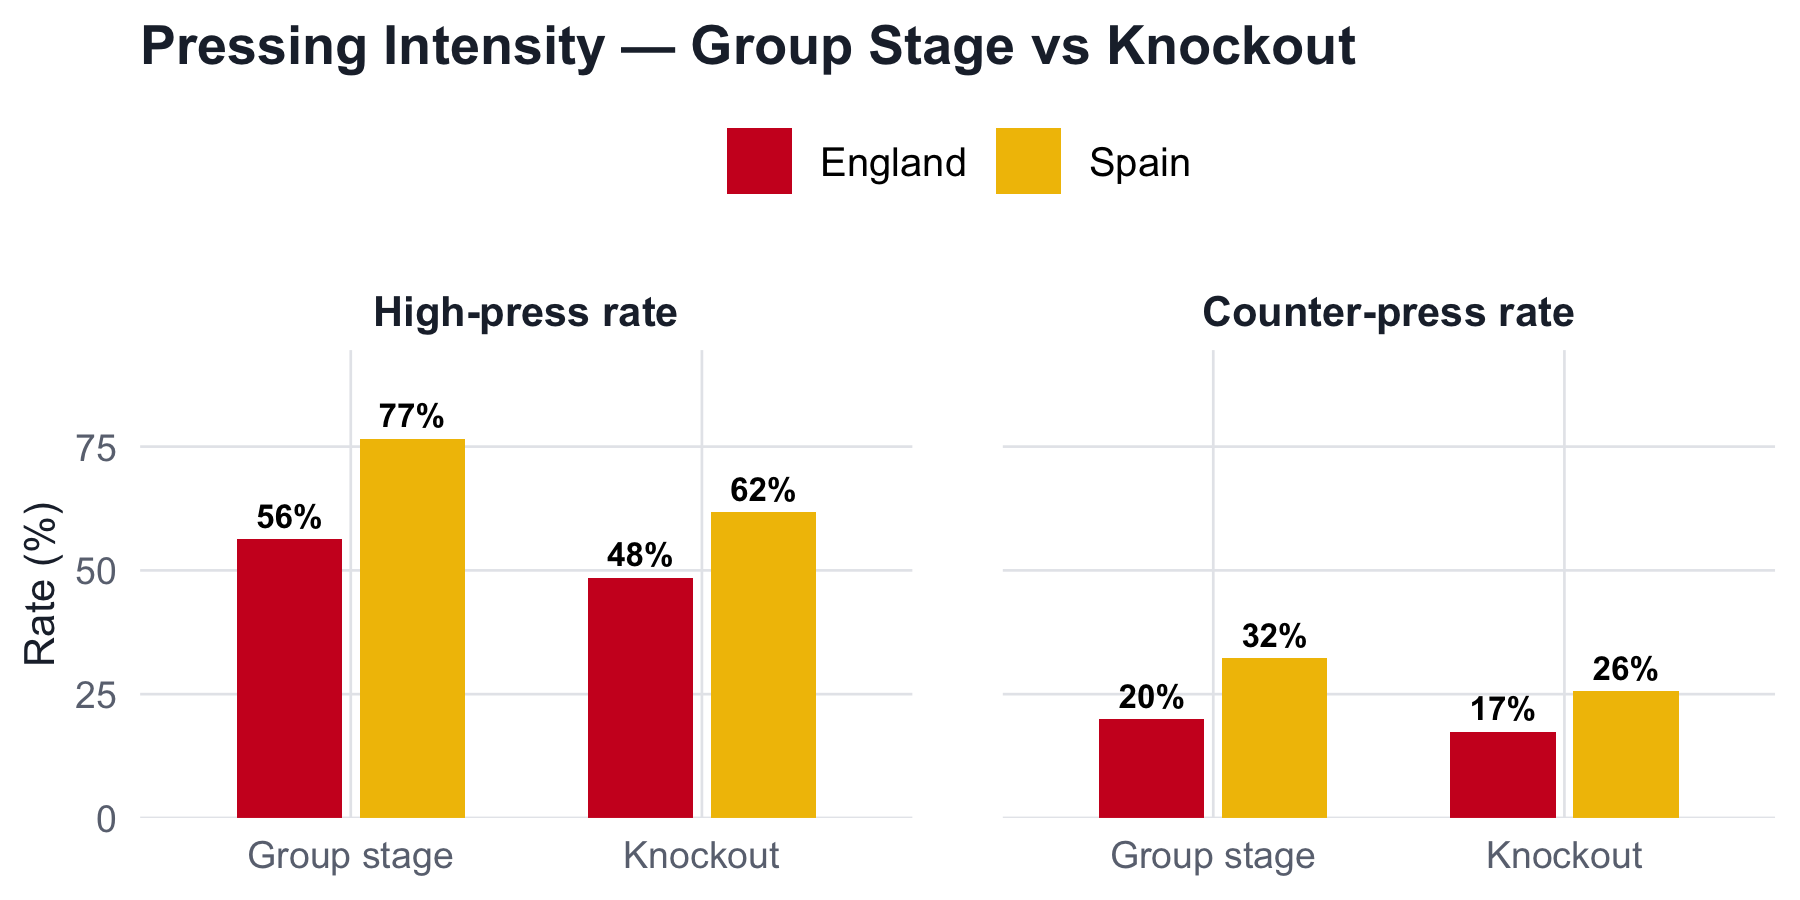
\includegraphics[keepaspectratio]{Report_files/figure-pdf/fig-pressing-1.png}}

}

\caption{\label{fig-pressing}Pressing intensity by stage --- high press
rate and counter-press rate for England and Spain across group stage and
knockout rounds. Spain pressed higher at every stage.}

\end{figure}%

\subsection{The Final}\label{the-final}

Looking at the attacking output in the final, Spain clearly dominated
England on both analysed metrics. Figure~\ref{fig-shot-map} shows Spain
had 23 shots compared to England's 8, demonstrating their will to create
attacking threat. The location of Spain's attempts was also more
centrally located around the penalty area, compared to England's more
dispersed shot ranges. Both goals in the match were headers. Spain's
Caldentey headed in from close range in the 24th minute (0.396 xG),
while England's Russo equalised with a header in the 56th minute (0.213
xG).

\begin{figure}

\centering{

\pandocbounded{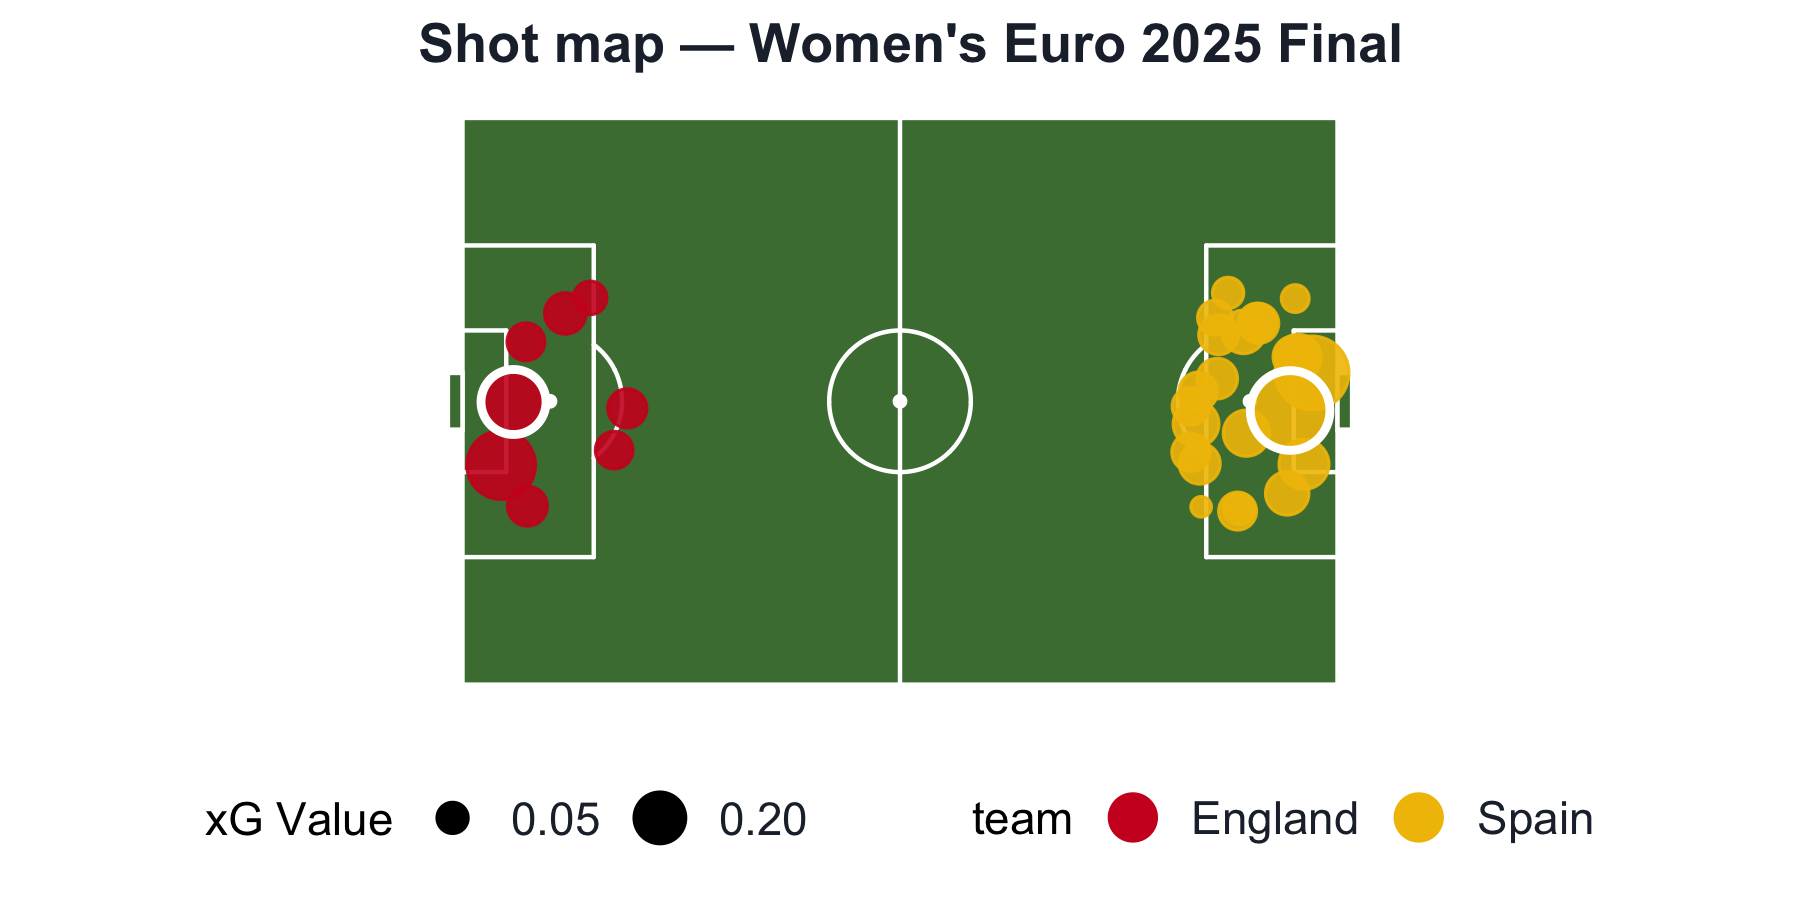
\includegraphics[keepaspectratio]{Report_files/figure-pdf/fig-shot-map-1.png}}

}

\caption{\label{fig-shot-map}Shot map for the Women's Euro 2025 Final.
England attack from the left, Spain attack from the right. Circle size
represents xG value. White ring indicates a goal. Spain registered 23
shots to England's 8.}

\end{figure}%

As further shown in Figure~\ref{fig-xg-timeline}, Spain was dominating
the attack from the opening minutes of the match, accumulating a total
of 2.14 xG across their 23 shots by the end of extra time. England only
reached a total xG of 0.88 from their 8 shots, but having a higher xG
per shot (0.11 xG vs 0.09 xG). England recorded their last shot in the
68th minute, meaning that they created no further chances during the
final 52 minutes of the match, including extra time. However, despite
this xG gap, the match ended 1-1 after 120 minutes, with England winning
3-1 on penalties.

\begin{figure}

\centering{

\pandocbounded{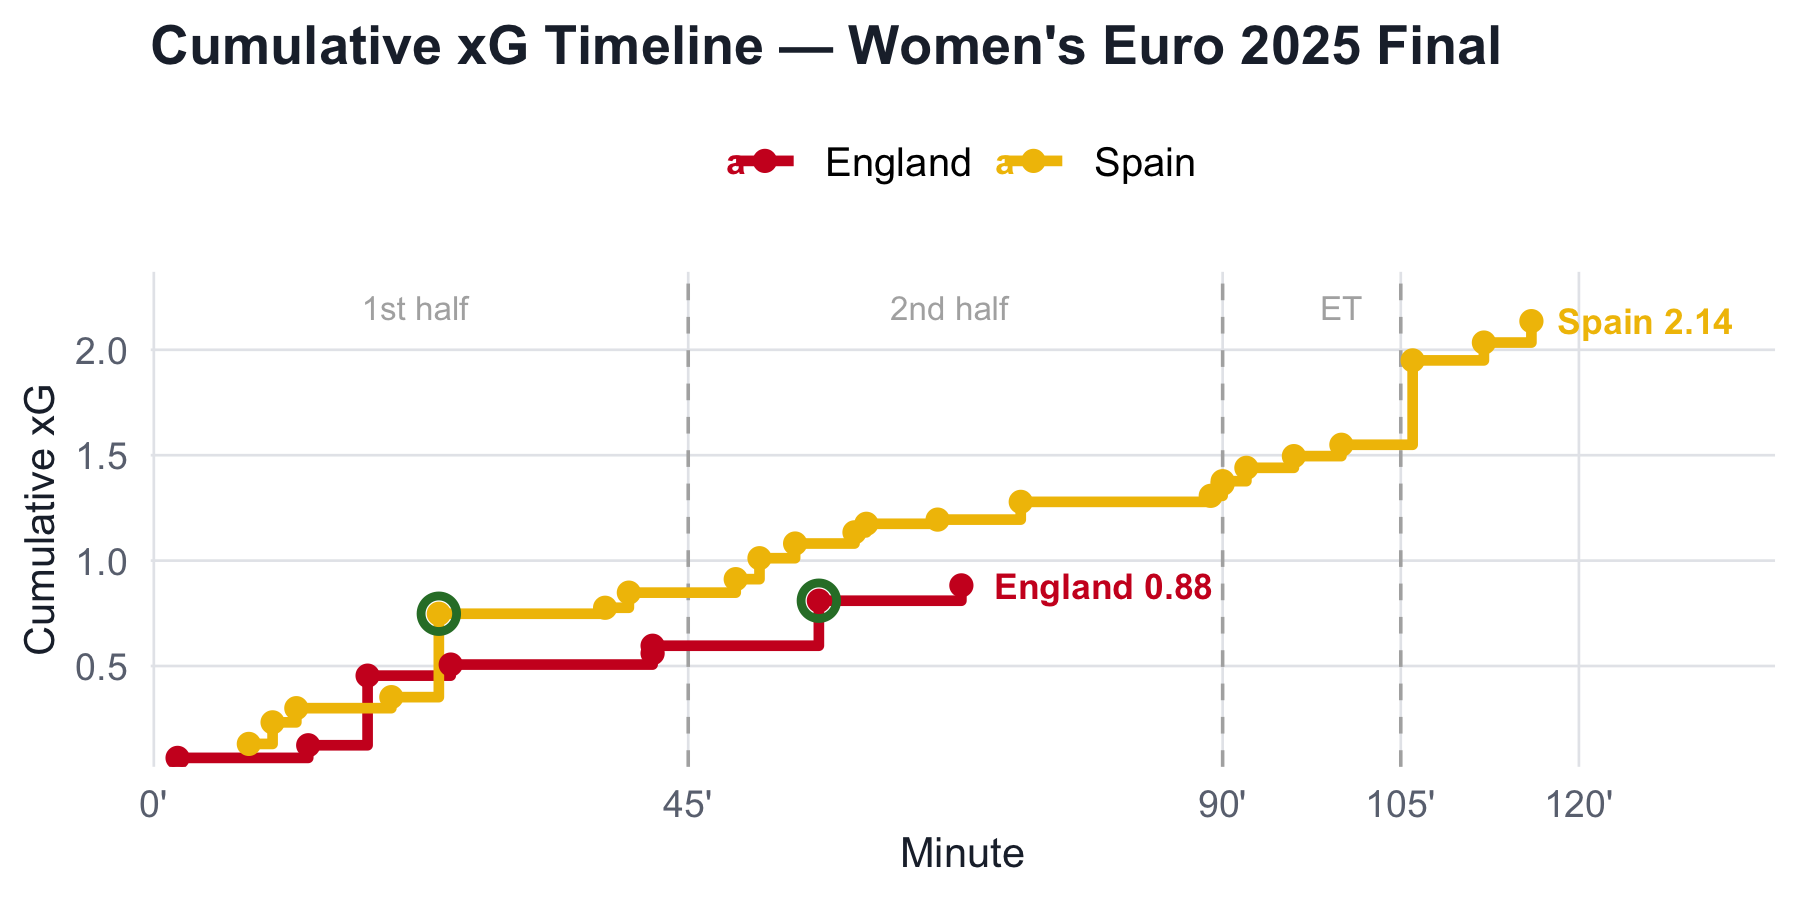
\includegraphics[keepaspectratio]{Report_files/figure-pdf/fig-xg-timeline-1.png}}

}

\caption{\label{fig-xg-timeline}Cumulative xG Timeline for the Women's
Euro 2025 Final. Spain dominated throughout, finishing with 2.14 xG.
England's last shot was in the 68th minute. Green rings indicate goals.}

\end{figure}%

When looking at the possession in the final, a few things stand out.
First, Spain dominated the pass distribution into the attacking third of
the pitch (29.2\%) compared to England's 15.2\% as shown in
Figure~\ref{fig-pass-thirds}. England, however, made more passes within
the defensive area of the pitch (37\% vs 22.5\%). This data illustrates
Spain did not only had more shots, but also attempted to create more
attacking threat as a team, showcasing their drive to win the match.
Whereas, England's defensive dominance reflects their more conservative
and compact approach in the final.

\begin{figure}

\centering{

\pandocbounded{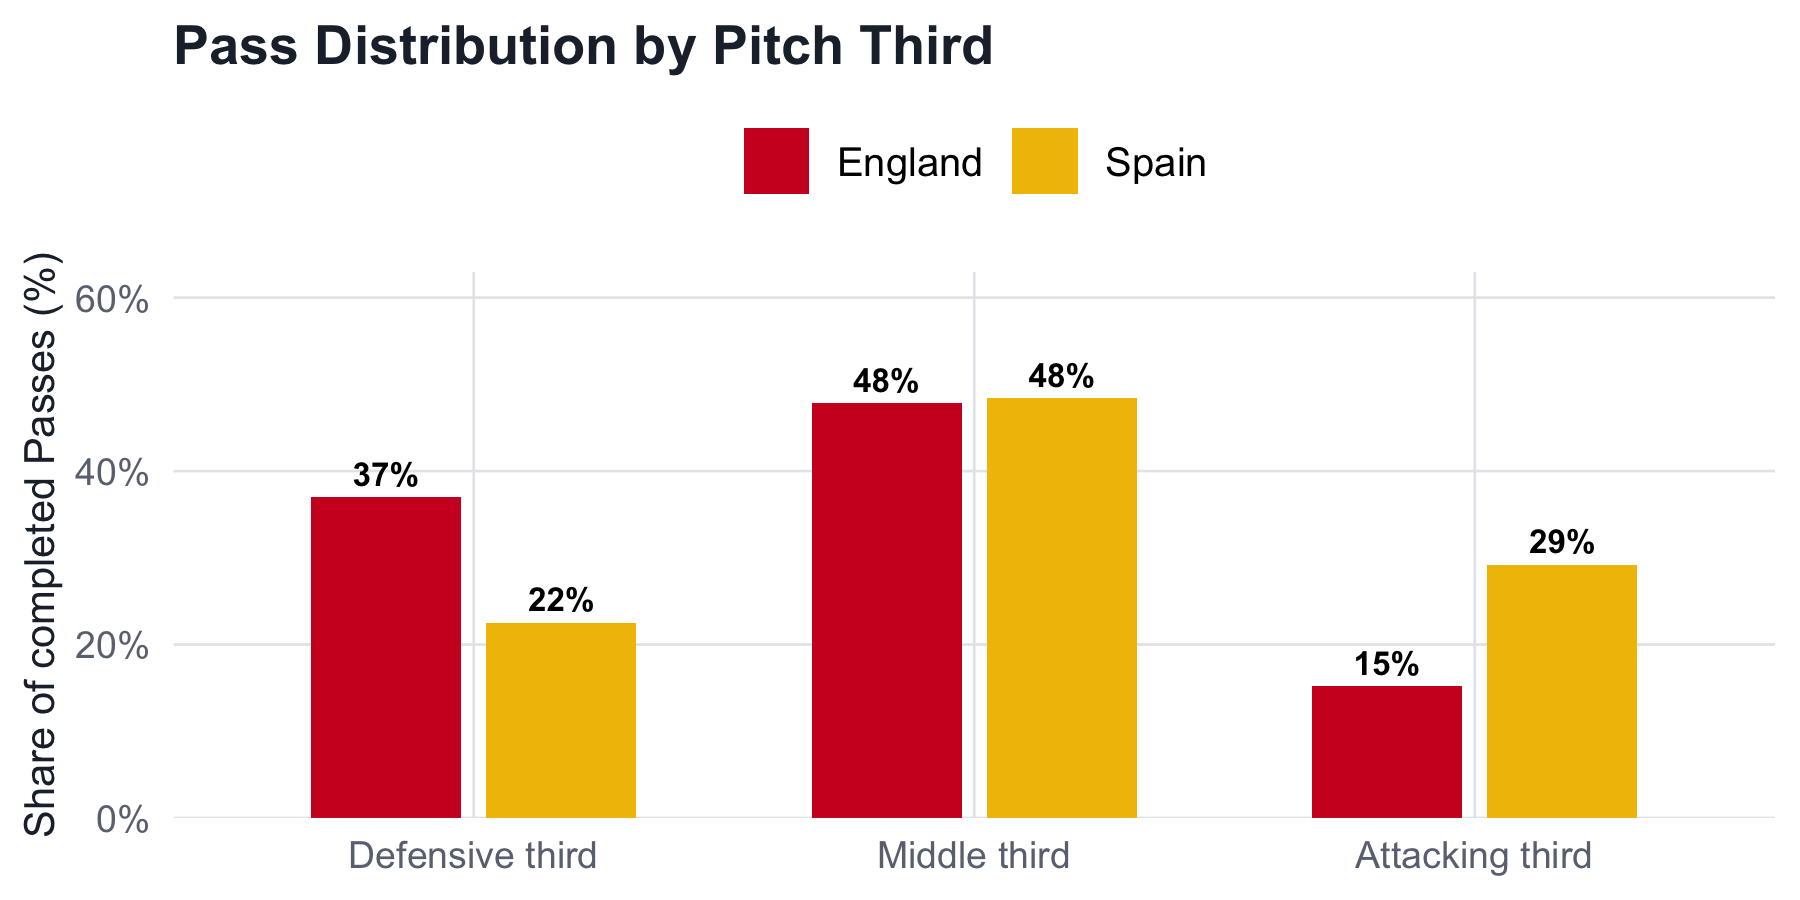
\includegraphics[keepaspectratio]{Report_files/figure-pdf/fig-pass-thirds-1.png}}

}

\caption{\label{fig-pass-thirds}Completed pass distribution by pitch
third in the final. Spain directed more passes into the attacking third,
while England were more concentrated in the defensive third.}

\end{figure}%

When looking at the most creative players for each team in the Final,
there are also clear differences between Bonmatí's (Spain) and Hemps'
(England) final-third actions. Despite both players playing the full 120
minutes, Bonmatí generated significantly more individual attacking
threat. As shown in Figure~\ref{fig-passmap}, Bonmatí operated across
the full width of the attacking third, completing final-third passes and
carries from both central and wide positions. Hemp's actions were more
concentrated on the left channel, which further reflects England's more
conservative and positionally disciplined attacking approach.

\begin{figure}

\centering{

\pandocbounded{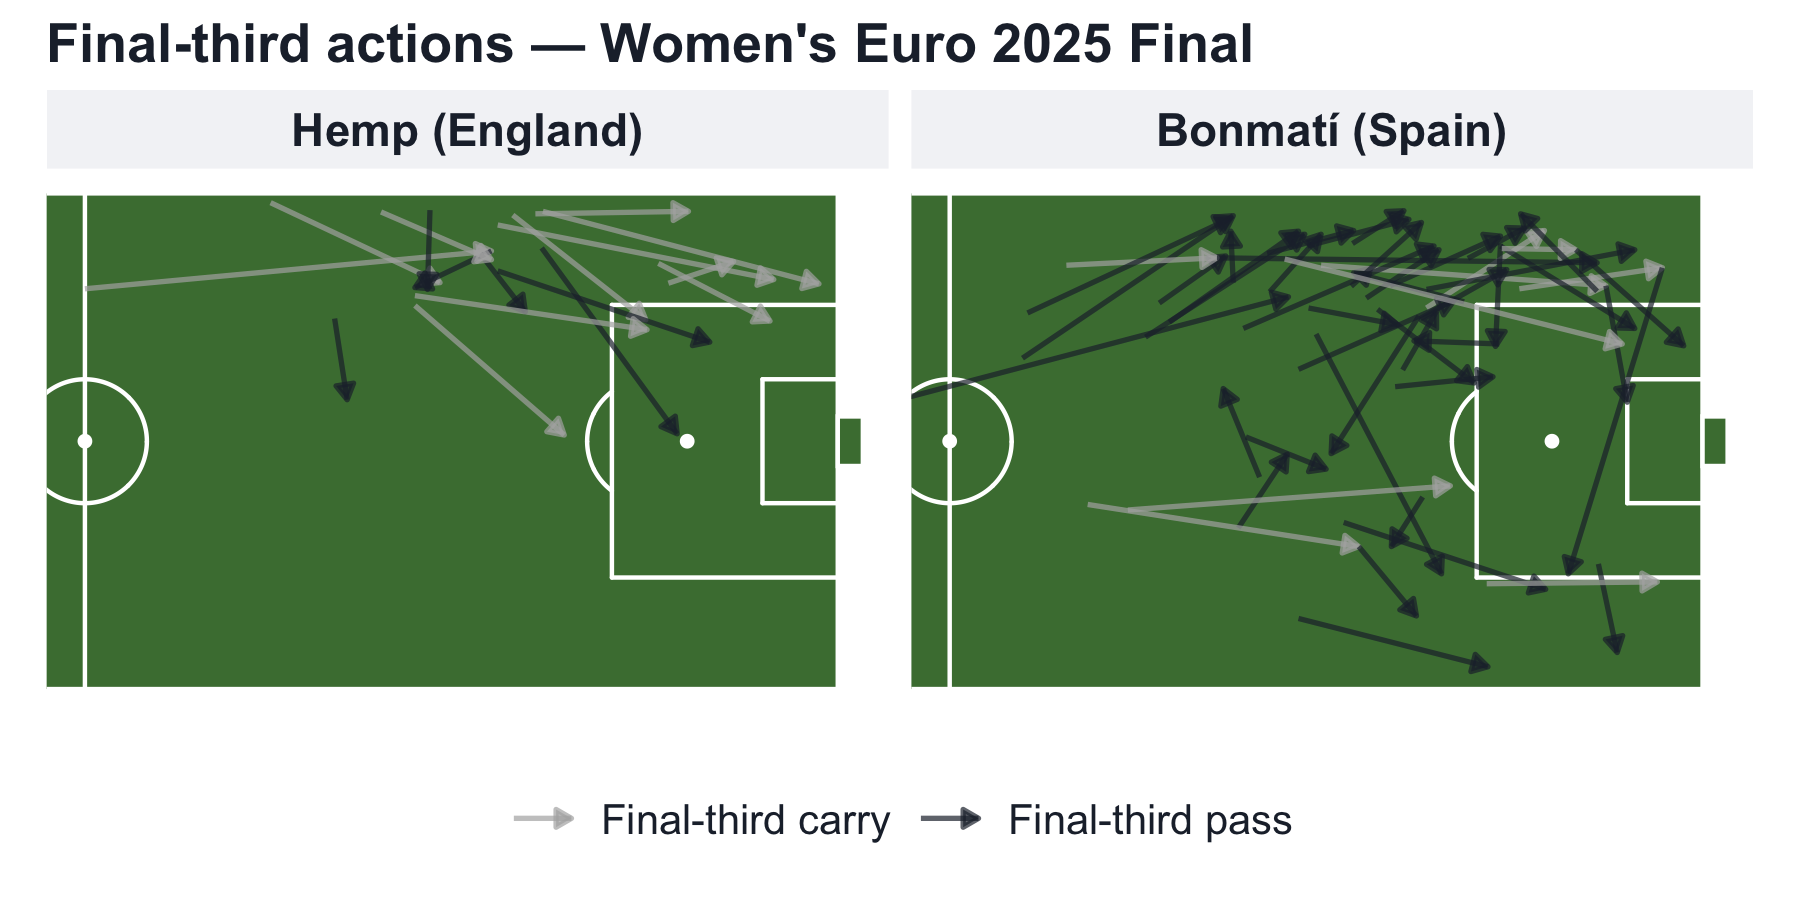
\includegraphics[keepaspectratio]{Report_files/figure-pdf/fig-passmap-1.png}}

}

\caption{\label{fig-passmap}Final-third actions for Bonmatí (Spain) and
Hemp (England) in the final. Arrows show completed passes and carries
ending in the final third. Bonmatí operated across the full width of the
attacking third while Hemp was concentrated through the left channel.}

\end{figure}%

\subsection{Analytical Outcome}\label{analytical-outcome}

As shown in Table~\ref{tbl-verdict} Spain led England on all seven
performance metrics across the tournament. Spain averaged 2.65 xG per
match compared to England's 2.45, while conceding considerably less
(0.67 vs 1.25 xG per match). Moreover, their pass completion was notably
higher (87.2\% vs 79.4\%). Pass completion only, however, does not
directly mean better possession. But, Spain showed their attacking
threat through other metrics. Particularly, for final third carries
Spain had a 6.6 percentage point lead compared to England. Consequently,
by attacking more, this also led to less shots faced per match (8.7 vs
11.8).

One finding that complicates this picture is England's pressing in the
final itself. England applied 393 pressures compared to Spain's 253,
even though Spain had a significantly higher high press rate across the
tournament (67.8\% vs 51.5\%). This suggests that England's tactical
approach in the final was more aggressive than the xG gap implies and
their defensive resilience was a key factor. However, based on the data,
Spain were the stronger side across all seven tournament-wide metrics.

\begin{longtable}[]{@{}llcc@{}}

\caption{\label{tbl-verdict}Key performance metrics --- England vs Spain
across the tournament. Spain led on all seven metrics.}

\tabularnewline

\toprule\noalign{}
Dimension & Metric & England & Spain \\
\midrule\noalign{}
\endhead
\bottomrule\noalign{}
\endlastfoot
Chance quality & Avg xG per match & 2.45 & \textbf{2.65} \\
Defensive Solidity & Avg xG conceded per match & 1.25 & \textbf{0.67} \\
Game control & High press rate (\%) & 51.50 & \textbf{67.8} \\
Game control & Pass completion (\%) & 79.40 & \textbf{87.2} \\
Attacking Threat & Final third carry rate (\%) & 29.10 &
\textbf{35.7} \\
Attacking Threat & Final third pass rate (\%) & 34.70 & \textbf{37.9} \\
Defensive Solidity & Shots faced per match & 11.80 & \textbf{8.7} \\

\end{longtable}

\section{Discussion, Limitations, and
Conclusion}\label{discussion-limitations-and-conclusion}

\subsection{Implication of Findings}\label{implication-of-findings}

The data clearly shows that Spain were the stronger team across the UEFA
Women's Euro 2025. The were performing better on all seven performance
metrics analysed, generated more xG per match (2.65 vs 2.45), conceded
considerably less (0.67 vs 1.25), on average across all stages of the
competition pressed higher and more aggressively. Especially in the
final the gap in chances created was significant. Spain created 2.14 xG
from 23 shots, while England only attempted 8 shots (0.88 xG) and the
last shot of the game coming in the 68th minute. Looking at these
conventional metrics, Spain deserved to win.

However, England managed to get a draw after extra time and then beating
Spain on penalties 3-1. This contradiction is what makes the result
analytically interesting. In the final, England recorded 393 pressures,
compared to Spain's 253. That suggests England took a tactically
deliberate defensive approach, absorb Spain's attacking pressure,
limiting their space and stay compact rather than dominating possession
and going forward. Their pass distribution further confirms this
approach, as it was mainly concentrated in the defensive and middle
thirds. The result shows what is regularly observed in football, where
match outcomes are heavily influenced by randomness and may not always
reflect underlying team performance (Brechot and Flepp, 2020).

This dashboard offers insights for a variety of football stakeholders.
For an analyst, the dashboard can be used as a framework to evaluate
whether tournament results reflect underlying performance. A coach can
use the pressing and ball progression data as a basis for the tactical
analysis to prepare for upcoming games. Due to the strength of both
England and Spain, it is not unlikely they will face each other again in
high-stake situations. By observing past patterns they can identify
potential strengths and weaknesses in their own team's and the
opponent's to help prepare the tactics based on the learned outcome from
this tournament. A journalist would be most interested in the xG
timeline for the final as a visualisation of the story. Spain dominated
for 120 minutes, England endured the pressures and in the end penalties
decided a match that the statistics alone cannot explain.

\subsection{Limitations}\label{limitations}

Despite the dashboard providing detailed insights into performance
metrics during the Women's Euros 2025, several limitations should be
acknowledged within the scope of the work. First, this analysis only
focused on on-ball event data. Any movements off the ball, such as
defensive shape and physical metrics like distance covered or sprint
intensity were not covered and therefore outside the scope of this
analysis. Especially England's defensive organisation in the final
cannot be fully quantified through the metrics used in this analysis.

Second, small sample sizes have an impact on the metrics. The maximum of
matches a team could play was six, and this only if the team went
through to the final. Majority of the teams only played three games
(group stage), or potentially one or two extra games in the knockout
stages. For example, England's xG figures are visibly inflated by their
6-1 win against Wales in the group stage, and vice versa Wales' average
xG difference (-2.65) is disproportionately negative for the same
reason. Averaging across six matches does produce useful comparisons,
but should be interpreted with caution due to the sample size and games
played for each team.

Finally, the player-level analysis was limited to two players (Bonmatí
and Hemp) due to them having the highest-volume of final-third actions
for their respective teams. This was a deliberate choice, but it
excludes contributions from other key players. For example, England's
Goalkeeper Hannah Hampton was named player of the match in the final
(UEFA, 2025b). (UEFA, 2025b). This shows that she had an influential
role in England's defence in the final and the penalty shootout, which
helped them retain their European title.

\subsection{Future Outlook}\label{future-outlook}

There are several extensions to this analysis to further strengthen it.
For example, the StatsBomb freeze frame data would help allowing to
evaluate shot quality with more precision by accounting for goalkeeper
positioning and defensive pressure at the moment of each attempt.
Additionally, physical tracking data, if available, could be
incorporated. This would strengthen the analysis to quantify for
example, England's defensive shape rather than implying it. Another
addition could be to extend the same analysis to other international
tournaments, such as the 2022 Women's Euro or the 2023 World Cup. This
could help in contextualise England's and Spain's 2025 performances
against their own historical benchmarks. Finally, an analysis that
includes the state of the match for each game, showing whether a team
was winning, drawing, or losing could be helpful. It would allow to
highlight deliberate tactical decisions in changes of play in attack and
defence. This would be particularly interesting to interpret England's
second-half and extra time pressing in the final to illustrate how they
were able to keep the result at 1-1 without attempting to shoot
themselves.

\subsection{Conclusion}\label{conclusion}

Returning to the opening question of whether England deserved to win the
Women's Euro 2025, the analysed data suggests they did not, at least not
on the basis of performance. Spain were dominating throughout the
tournament and in the final, and the analysed metrics support that
conclusion in their favour. England were able to retain their title by
having a high tactical discipline, clinical finishing under pressure as
well as penalty shootout success. All that matters a lot in a knockout
tournament, where the state of the game can shift from one moment to the
other. However, not all of those factors can be fully capture by event
data alone.

However, the data does not discriminate England's achievement to win the
title. Winning a major tournament depends on various elements and
requires both performance and results. England sustained under pressure
when it mattered the most. However, it does suggest that the scoreline,
and the trophy only tell one part of the story. The dashboard was built
to tell the other part.

\newpage{}

\section*{List of Tools Used}\label{list-of-tools-used}
\addcontentsline{toc}{section}{List of Tools Used}

Anara Technologies (2026) \emph{Anara} (Pro Version). Available at:
\url{https://anara.com}

\begin{itemize}
\tightlist
\item
  Assisted in understanding and summarising academic literature
\item
  Facilitated the organisation of research findings
\end{itemize}

Anthropic (2026) \emph{Claude} (Version claude-sonnet-4-6). Available
at: \url{https://claude.ai}

\begin{itemize}
\tightlist
\item
  Assisted in debugging R code and Shiny app development
\item
  Support with structuring report sections
\item
  Proofreading and grammar check for cohesion and readability
\end{itemize}

Grammarly Inc.~(2026) \emph{Grammarly} (Free Version). Available at:
\url{https://www.grammarly.com}

\begin{itemize}
\tightlist
\item
  Support with spelling and grammar checks, including punctuation and
  preposition use
\end{itemize}

QuillBot (2026) \emph{Paraphrasing Tool} (Free Version). Available at:
\url{https://quillbot.com/paraphrasing-tool}

\begin{itemize}
\tightlist
\item
  Assisting with paraphrasing sentences and sentence structures
\item
  Finding synonyms
\end{itemize}

Zotero (2026) \emph{Zotero} (MacOS Version). Available at:
\url{https://www.zotero.org/}

\begin{itemize}
\tightlist
\item
  Assisting in the organisation of references and citations
\end{itemize}

\newpage{}

\section*{Appendices}\label{appendices}
\addcontentsline{toc}{section}{Appendices}

\subsection*{Appendix A: Dashboard
Preview}\label{appendix-a-dashboard-preview}
\addcontentsline{toc}{subsection}{Appendix A: Dashboard Preview}

\newpage{}

\section*{References}\label{bibliography}
\addcontentsline{toc}{section}{References}

\phantomsection\label{refs}
\begin{CSLReferences}{0}{1}
\bibitem[\citeproctext]{ref-bransenDavis2024}
Bransen, L. and Davis, J. (2024) {``A data-driven analysis of the
technical and tactical evolution of elite women's football,''}
\emph{International Journal of Sports Science \& Coaching}, 19(6), pp.
2449--2459. Available at:
\url{https://doi.org/10.1177/17479541241257809}.

\bibitem[\citeproctext]{ref-brechotFlepp2020}
Brechot, M. and Flepp, R. (2020) {``Dealing with randomness in match
outcomes: How to rethink performance evaluation in european club
football using expected goals,''} \emph{Journal of Sports Economics},
21(4), pp. 335--362. Available at:
\url{https://doi.org/10.1177/1527002519897962}.

\bibitem[\citeproctext]{ref-dorrington2025}
Dorrington, N. (2025) \emph{Pressure data in football: Recruitment and
opposition analysis applications}. Hudl Statsbomb. Available at:
\url{https://www.hudl.com/blog/pressure-data-football-statsbomb}
(Accessed: May 7, 2026).

\bibitem[\citeproctext]{ref-hudlNoDate}
Hudl (no date) \emph{Access statsbomb data with StatsbombR}. Hudl
Support. Available at:
\url{https://support.hudl.com/s/article/access-statsbomb-data-statsbombr}
(Accessed: April 23, 2026).

\bibitem[\citeproctext]{ref-hudlStatsbomb2021}
Hudl Statsbomb (2021) \emph{StatsBomb data case studies: Freeze frames
and defender locations}. Available at:
\url{https://blogarchive.statsbomb.com/news/statsbomb-data-case-studies-freeze-frames-and-defender-locations/}
(Accessed: May 7, 2026).

\bibitem[\citeproctext]{ref-hudlStatsbomb2024}
Hudl Statsbomb (2024) \emph{Hudl and StatsBomb combine expertise to
transform advanced data analytics}. Hudl. Available at:
\url{https://www.hudl.com/blog/hudl-statsbomb} (Accessed: May 7, 2026).

\bibitem[\citeproctext]{ref-hudlStatsbombNoDate}
Hudl Statsbomb (no date) \emph{The world's most advanced football data
for professional teams}. Hudl. Available at:
\url{https://www.hudl.com/en_gb/products/statsbomb} (Accessed: May 7,
2026).

\bibitem[\citeproctext]{ref-sanders2025}
Sanders, E. (2025) \emph{England 1-1 spain: Lionesses retain title with
dramatic penalty victory as chloe kelly score winning kick}. BBC Sport.
Available at:
\url{https://www.bbc.co.uk/sport/football/live/c78n2p6yz3lt} (Accessed:
May 7, 2026).

\bibitem[\citeproctext]{ref-sievert2023}
Sievert, C. (2023) \emph{Towards easy, delightful, and customizable
dashboards in shiny for r with {bslib}}. Shiny. Available at:
\url{https://shiny.posit.co/blog/posts/bslib-dashboards/} (Accessed: May
8, 2026).

\bibitem[\citeproctext]{ref-statsbomb2019}
StatsBomb (2019) \emph{StatsBomb open data specification v1.1}.
Available at:
\url{https://github.com/statsbomb/open-data/blob/master/doc/StatsBomb\%20Open\%20Data\%20Specification\%20v1.1.pdf}
(Accessed: April 30, 2026).

\bibitem[\citeproctext]{ref-statsbomb2022}
StatsBomb (2022) \emph{Accessing \& working with StatsBomb data in r}.
Available at:
\url{https://blogarchive.statsbomb.com/uploads/2022/08/Working-with-R.pdf}
(Accessed: April 30, 2026).

\bibitem[\citeproctext]{ref-tjonndal2024}
Tjønndal, A. \emph{et al.} (2024) {``"Women play football, not women's
football": The potentials and paradoxes of professionalisation expressed
at the UEFA women's EURO 2022 championship,''} \emph{European Journal
for Sport and Society}, 21(3), pp. 276--294. Available at:
\url{https://doi.org/10.1080/16138171.2024.2306443}.

\bibitem[\citeproctext]{ref-uefaTeamTournament2025}
UEFA (2025a) \emph{England and spain dominate UEFA women's EURO 2025
team of the tournament}. UEFA.com. Available at:
\url{https://www.uefa.com/womenseuro/news/029b-1e58468918c0-bc98c43b7716-1000--england-and-spain-dominate-uefa-women-s-euro-2025-team-of/}
(Accessed: May 7, 2026).

\bibitem[\citeproctext]{ref-uefaHampton2025}
UEFA (2025b) \emph{Hannah hampton named women's EURO 2025 final player
of the match}. UEFA.com. Available at:
\url{https://www.uefa.com/womenseuro/news/029b-1e56a18fd1e8-7b0ee2b3f430-1000--hannah-hampton-named-women-s-euro-2025-final-player-of-the-/}
(Accessed: May 7, 2026).

\bibitem[\citeproctext]{ref-uefaTopScorer2025}
UEFA (2025c) \emph{Women's EURO 2025 top scorer: Esther gonzález}.
UEFA.com. Available at:
\url{https://fr.uefa.com/womenseuro/news/029b-1e267b829acd-2950e41eb1a6-1000--women-s-euro-2025-top-scorer-esther-gonzalez/}
(Accessed: May 7, 2026).

\bibitem[\citeproctext]{ref-uefaRecords2025}
UEFA (2025d) \emph{Women's EURO 2025: All the records set in
switzerland}. UEFA.com. Available at:
\url{https://www.uefa.com/womenseuro/news/029b-1e3dbb1ab3fe-1fadb3a596e8-1000--women-s-euro-2025-all-the-records-set-in-switzerland/}
(Accessed: May 7, 2026).

\bibitem[\citeproctext]{ref-womensSportTrust2026}
Women's Sport Trust (2026) \emph{The visibility of women's sport hit new
highs in 2025}. Womens Sport Trust. Available at:
\url{https://www.womenssporttrust.com/the-visibility-of-womens-sport-hit-new-highs-in-2025/}
(Accessed: May 7, 2026).

\end{CSLReferences}




\end{document}
